\documentclass{article}

% if you need to pass options to natbib, use, e.g.,:
%     \PassOptionsToPackage{numbers, compress}{natbib}
% before loading neurips_2021

% ready for submission
\usepackage[preprint]{neurips_2023}

% to compile a preprint version, e.g.,, for submission to arXiv, add add the
% [preprint] option:
%     \usepackage[preprint]{neurips_2021}

% to compile a camera-ready version, add the [final] option, e.g.,:
%     \usepackage[final]{neurips_2021}

% to avoid loading the natbib package, add option nonatbib:
%    \usepackage[nonatbib]{neurips_2021}

\usepackage[utf8]{inputenc} % allow utf-8 input
\usepackage[T1]{fontenc}    % use 8-bit T1 fonts
\usepackage[colorlinks=true]{hyperref}       % hyperlinks
\usepackage{url}            % simple URL typesetting
\usepackage{booktabs}       % professional-quality tables
\usepackage{amsfonts}       % blackboard math symbols
\usepackage{nicefrac}       % compact symbols for 1/2, etc.
\usepackage{microtype}      % microtypography
\usepackage{xcolor}         % colors
\usepackage{graphicx}       % for images
\title{Predicting YouTube Video Views \\from Video and Thumbnail Features}

% The \author macro works with any number of authors. There are two commands
% used to separate the names and addresses of multiple authors: \And and \AND.
%
% Using \And between authors leaves it to LaTeX to determine where to break the
% lines. Using \AND forces a line break at that point. So, if LaTeX puts 3 of 4
% authors names on the first line, and the last on the second line, try using
% \AND instead of \And before the third author name.

\author{%
  Lean Ting Jin\\
  Matrikelnummer 6956985\\
  \texttt{ting-jin.lean@student.uni-tuebingen.de} \\
  \And
  Finn Springorum\\
  Matrikelnummer 6124977\\
  \texttt{finn.springorum@student.uni-tuebingen.de} \\
  \And
  Christian Traxler\\
  Matrikelnummer 6969273\\
  \texttt{christian.traxler@student.uni-tuebingen.de} \\
  \And
  Anna Chechenina\\
  Matrikelnummer 6987499\\
  \texttt{dummymail1@uni-tuebingen.de} \\
}

\begin{document}

\maketitle

\begin{abstract}
  We are are planning to use the YouTube Data API v3 \cite{youtubeapi} to see which factors of a YouTube video best predict how many videos it will receive. 

\end{abstract}

\section{Introduction}
YouTube is the second most visited website in the world. In 2024, creators uploaded $x$ hours of content to YouTube, and were paid a total of \$$y$ million in revenue (source: \cite{}). For YouTube creators, there is a massive financial incentive to maximize a video's view count.

The view count of a video depends on the YouTube algorithm. However, this algorithm is a black box. Despite this, it is widely believed that the number of views a video receives is strongly correlated with 3 main factors: (1) the click-through rate of the video's thumbnail, (2) the watch duration of the video and (3) the number of subscribers of the channel (source: \cite{}).


Increasing the watch duration of a video requires a significant investment in time and money. Meanwhile, the number of subscribers a channel has is also beyond the control of a creator. In contrast, it is easier for a creator to tweak the thumbnail of a video to try to improve the click-through rate. While multiple online resources \cite{}, and prominent YouTubers \cite{} claim that more eye-catching thumbnails get more clicks, there does not seem to be any quantitative results on this topic in literature.


Admittedly, it is not clear how one can quantify the eye-catchiness of a thumbnail. However, it is reasonable to assume certain features such as image color, saturation and the presence of human faces are important. Therefore, the aim of this study is to investigate the relationship between the eye-catchiness of a video's thumbnail, and the number of views it receives. As a proxy for eye-catchiness, we use 6 features which are easily derived from the thumbnail: hue, saturation, lightness, contrast, sharpness and the number of faces.


\section{Methods}
\textbf{Data Collection.} We used the YouTube Data API \cite{youtubeapi} to collect data on videos from a variety of categories. There are 15 main categories of videos on YouTube. Given our interest in thumbnails, we decided to focus on video categories intended to appear in the feed of a user and elicit a response, which are: Comedy, Education, Entertainment, Gaming, How-to \& Style, News \& Politics, People and Blogs, and Sports.

We excluded videos explicitly sought after through searches (e.g., Film \& Animation), videos which are unlikely to include human faces on their thumbnail (e.g., Pets \& Animals), or videos from a very niche field (e.g., Nonprofits \& Activism).

Due to the limited number of videos that can be retrieved for a given query, the date range from January 1st, 2015 to the time of collection was divided into disjoint sets, and 500 videos were requested for each period. This strategy enabled the acquisition of thousands of videos for a single query. To prevent duplicates while respecting the daily API limit, our data collection strategy entailed the request of up to 2,500 videos from a designated category, each accompanied by a singular generic keyword (e.g., most popular video games for the Gaming category), until the collection comprised precisely 10,000 unique videos from said category, yielding a dataset with 8 categories, for a total of 80,000 unique videos.



\textbf{Video and Thumbnail Features.} For each video $V_i$, we obtained the following information of interest: thumbnail, $T_i$, view count, $N_i$ and subscriber count, $S_i$. From each thumbnail $T_{i}$, we extracted the following 6 features: hue ($h_{i}$), saturation ($s_{i}$), lightness ($l_{i}$), contrast ($c_{i}$), sharpness ($s_{i}$) and number of faces ($f_{i}$).

The hue is the angle of the mean color of the thumbnail in the HSV color space, with a range of 0 to 360 degrees. The saturation, lightness and contrast follow their standard definitions as implemented in the OpenCV Python library (normalized to [0,1]). The sharpness is the log variance of the Laplacian of the grayscale image. The number of faces is the number of distinct faces in the thumbnail as predicted by RetinaFace model implemented in the DeepFace library \cite{serengil2024lightface,serengil2020lightface}.


\textbf{Analysis.} We are interested the the relationship between the view count $N_i$ and the 6 features derived from the thumbnail $T_i$. However, before performing any analysis, we note that intuitively, a video $V_i$ published by a channel with more subscribers $S_i$ is likely to have a higher view count $N_i$ compared to one with fewer subscribers, regardless of the thumbnail features. To remove this influence, we first fitted a linear regression model of (log) view count against (log) subscriber count. As the data appears log-normal, the base-10 logarithm is used to ensure that the residuals are homoscedastic and normally distributed. Only the residuals of this model, called the residual log view count, $R_{i} := \log(N_i) - \hat{\beta}_0^{(\gamma)} - \hat{\beta}_1^{(\gamma)} \log(S_i)$ were considered for the remainder of the analysis. $\gamma \in \{1, 2, \cdots, 8\}$ corresponds to one of the 8 categories that video $V_i$ belongs to.


\begin{figure}[h]
  \begin{minipage}[t]{0.45\textwidth}
    \vspace{0pt}  % Removes top spacing
    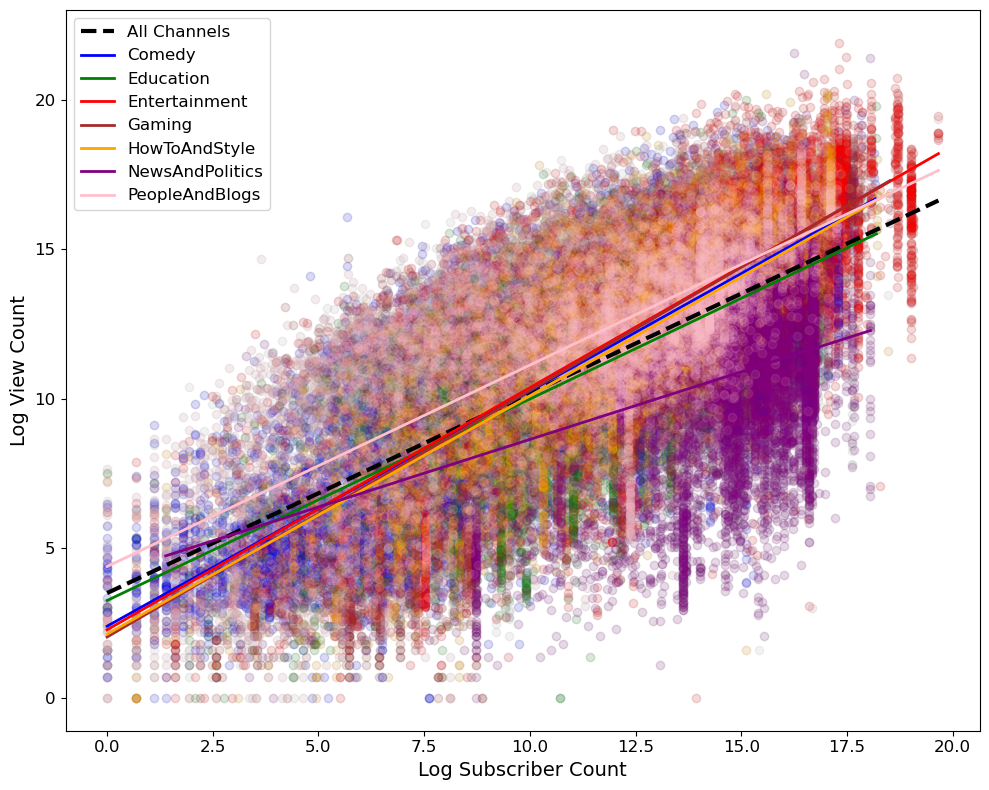
\includegraphics[width=\textwidth]{figs/subscriber.png}
  \end{minipage}%
  \hspace{0.05\textwidth}%
  \begin{minipage}[t]{0.45\textwidth}
    \vspace{0pt}  % Removes top spacing
    \caption{Regression of log view count against log subscriber count. The relationship is similar for all 8 video categories.
    For the combined dataset, the relationship is $\widehat{\log(N_i)} = \hat{\beta}_0 + \hat{\beta}_1 \cdot \log(S_i)$, 95\% CI for $\beta_0 = [3.445, 3.571]$, 95\% CI for $\beta_1 = [0.663, 0.673]$, $R^2 = 0.467$.}
    \label{fig:scatter_plot}

  \end{minipage}
\end{figure}




Next, the correlation between the 6 thumbnail features was investigated. There did not appear to be strong multicollinearity between features. A linear regression model was fitted to each continuous feature (saturation, lightness, contrast, sharpness).

Meanwhile, the number of faces $f_{i}$ was treated as a discrete feature, and 95\% confidence intervals of the residual log view count $R_{i}$ were computed for each face count $k\in\{0,1,2,3\}$. The videos with thumbnails containing 3 or more faces were grouped into the same bin and analyzed together.

We also treated the hue $h_{i}$ as a discrete feature. Since hue ranges from 0 to 360 degrees, we grouped the videos into 6 bins of equal width. For example, bin with a hue of 0-60 degrees would contain videos with reddish thumbnails. We then computed a 95\% confidence interval for $R_{i}$ for each bin.

Finally, a multiple linear regression model was fitted to the residual log view count $R_{i}$ against hue, saturation, lightness, contrast, and number of faces.

\section{Results}


\section{Discussion/Limitations}
\textbf{Discussion }

\textbf{Limitations } As a project based on the YouTube API, there are couple of inherent limitations of the data collection. One issue with the data collection is the categories: each video is either user-defined or automatically assigned only one category. This means that there exists some error in the categories such that errors are likely and that some categories that we wanted to exclude (like music videos) are likely to be included and may skew results. \\
Also, 


\section{Statement of Contributions}

\emph{Here is an example:}

XX performed the correlation analysis, organized the data and code for the processing of dataset1 and subdataset2, and created the scatter plot. 
YY created the random forest regression model, performed the data cleaning for the xyz analysis / xyz database, and created the bar charts to display the regression results. 
ZZ researched and collected the raw data, restructured the pipeline for the data analysis, and proof-read the draft for the final report. 
AA performed the data cleaning for dataset1, and performed the Ridge and Lasso regularization. 
All members of the group contributed to writing the report.



\bibliographystyle{unsrt}%Used BibTeX style is unsrt
\bibliography{bibliography}

\end{document}